%!TEX root = bachelor_thesis.tex

\chapter{Einleitung}

Ein Quasar ist der aktive Kern einer Galaxie, der im sichtbaren Bereich des Lichtes nahezu punktförmig (wie ein Stern) erscheint und sehr große Energiemengen in anderen Wellenlängenbereichen ausstrahlt. Er besteht aus einem Schwarzen Loch umgeben von einer Scheibe leuchtender Materie. Der Name Quasar leitet sich von \textit{quasi-stellar radio source} (‚sternartige Radioquelle‘) ab.

\begin{figure}[h]
	\centering
	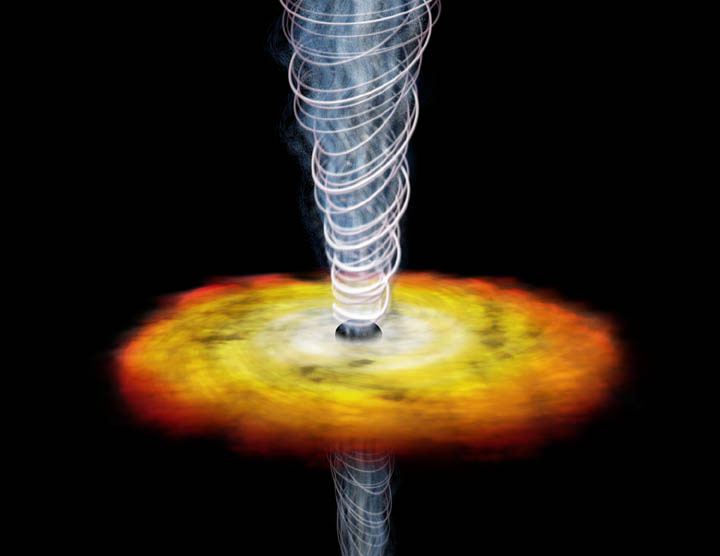
\includegraphics[width=10cm]{Imgs/quasar_illustration}
	\caption{Künstlerische Darstellung eines Quasars\cite{wikiQuasar1}}
	\label{fig:darstQuasar}
\end{figure}